\documentclass{standalone}
\usepackage{tikz}
\usetikzlibrary{patterns, positioning}

\begin{document}
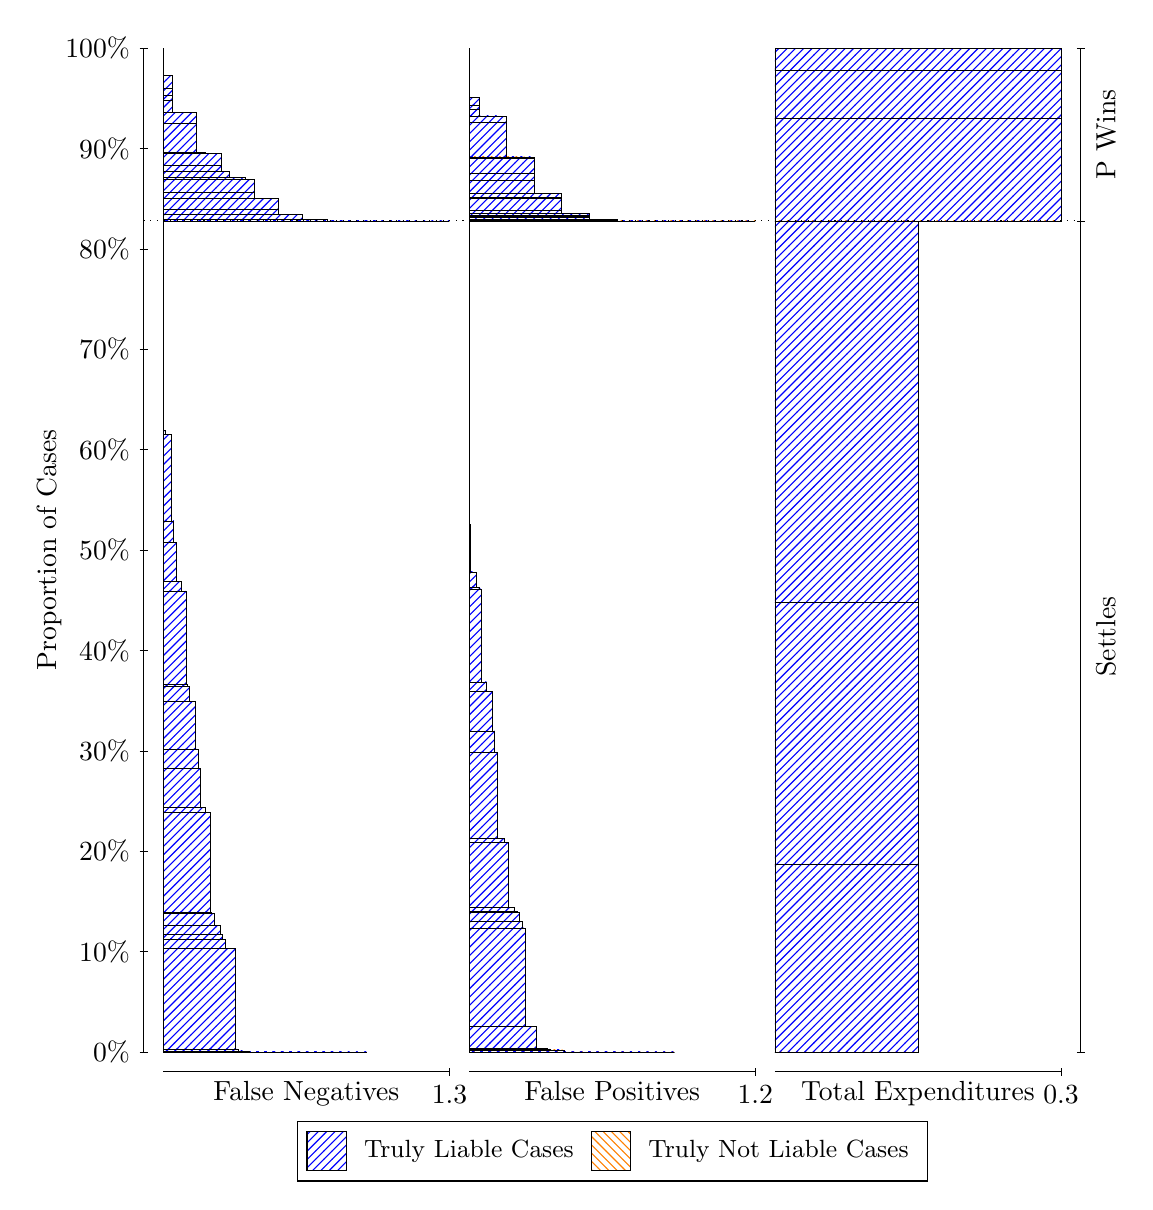
\begin{tikzpicture}
\draw[black, very thin] (1.5,1.75) -- (1.5,14.5);
\node[rotate=90, anchor=center] at (0.3, 8.125) {Proportion of Cases};
\draw[black, very thin] (1.45,1.75) -- (1.55,1.75);
\node[anchor=east] at (1.45, 1.75) {0\%};
\draw[black, very thin] (1.45,3.025) -- (1.55,3.025);
\node[anchor=east] at (1.45, 3.025) {10\%};
\draw[black, very thin] (1.45,4.3) -- (1.55,4.3);
\node[anchor=east] at (1.45, 4.3) {20\%};
\draw[black, very thin] (1.45,5.575) -- (1.55,5.575);
\node[anchor=east] at (1.45, 5.575) {30\%};
\draw[black, very thin] (1.45,6.85) -- (1.55,6.85);
\node[anchor=east] at (1.45, 6.85) {40\%};
\draw[black, very thin] (1.45,8.125) -- (1.55,8.125);
\node[anchor=east] at (1.45, 8.125) {50\%};
\draw[black, very thin] (1.45,9.4) -- (1.55,9.4);
\node[anchor=east] at (1.45, 9.4) {60\%};
\draw[black, very thin] (1.45,10.675) -- (1.55,10.675);
\node[anchor=east] at (1.45, 10.675) {70\%};
\draw[black, very thin] (1.45,11.95) -- (1.55,11.95);
\node[anchor=east] at (1.45, 11.95) {80\%};
\draw[black, very thin] (1.45,13.225) -- (1.55,13.225);
\node[anchor=east] at (1.45, 13.225) {90\%};
\draw[black, very thin] (1.45,14.5) -- (1.55,14.5);
\node[anchor=east] at (1.45, 14.5) {100\%};

\draw[black, very thin] (13.4,1.75) -- (13.4,14.5);
\draw[black, very thin] (13.35,1.75) -- (13.45,1.75);
\node[anchor=west] at (13.35, 1.75) {};
\draw[black, very thin] (13.35,12.305) -- (13.45,12.305);
\node[anchor=west] at (13.35, 12.305) {};
\draw[black, very thin] (13.35,14.5) -- (13.45,14.5);
\node[anchor=west] at (13.35, 14.5) {};

\draw[black, very thin, pattern color=blue, pattern=north east lines] (1.75,1.75) rectangle (4.3353,1.75);
\draw[black, very thin, pattern color=blue, pattern=north east lines] (1.75,1.75) rectangle (4.0558,1.75);
\draw[black, very thin, pattern color=blue, pattern=north east lines] (1.75,1.75) rectangle (4.0247,1.75);
\draw[black, very thin, pattern color=blue, pattern=north east lines] (1.75,1.75) rectangle (3.916,1.75);
\draw[black, very thin, pattern color=blue, pattern=north east lines] (1.75,1.75) rectangle (3.7763,1.75);
\draw[black, very thin, pattern color=blue, pattern=north east lines] (1.75,1.75) rectangle (3.7452,1.75);
\draw[black, very thin, pattern color=blue, pattern=north east lines] (1.75,1.75) rectangle (3.7142,1.75);
\draw[black, very thin, pattern color=blue, pattern=north east lines] (1.75,1.75) rectangle (3.6365,1.75);
\draw[black, very thin, pattern color=blue, pattern=north east lines] (1.75,1.75) rectangle (3.6055,1.75);
\draw[black, very thin, pattern color=blue, pattern=north east lines] (1.75,1.75) rectangle (3.4968,1.75);
\draw[black, very thin, pattern color=blue, pattern=north east lines] (1.75,1.75) rectangle (3.4657,1.75);
\draw[black, very thin, pattern color=blue, pattern=north east lines] (1.75,1.75) rectangle (3.4347,1.75);
\draw[black, very thin, pattern color=blue, pattern=north east lines] (1.75,1.75) rectangle (3.4036,1.75);
\draw[black, very thin, pattern color=blue, pattern=north east lines] (1.75,1.75) rectangle (3.326,1.75);
\draw[black, very thin, pattern color=blue, pattern=north east lines] (1.75,1.75) rectangle (3.2949,1.75);
\draw[black, very thin, pattern color=blue, pattern=north east lines] (1.75,1.75) rectangle (3.2173,1.75);
\draw[black, very thin, pattern color=blue, pattern=north east lines] (1.75,1.75) rectangle (3.1863,1.75);
\draw[black, very thin, pattern color=blue, pattern=north east lines] (1.75,1.75) rectangle (3.1552,1.7501);
\draw[black, very thin, pattern color=blue, pattern=north east lines] (1.75,1.7501) rectangle (3.1241,1.7501);
\draw[black, very thin, pattern color=blue, pattern=north east lines] (1.75,1.7501) rectangle (3.0931,1.7501);
\draw[black, very thin, pattern color=blue, pattern=north east lines] (1.75,1.7501) rectangle (3.0155,1.7506);
\draw[black, very thin, pattern color=blue, pattern=north east lines] (1.75,1.7506) rectangle (2.9844,1.7507);
\draw[black, very thin, pattern color=blue, pattern=north east lines] (1.75,1.7507) rectangle (2.9068,1.751);
\draw[black, very thin, pattern color=blue, pattern=north east lines] (1.75,1.751) rectangle (2.8757,1.751);
\draw[black, very thin, pattern color=blue, pattern=north east lines] (1.75,1.751) rectangle (2.8447,1.7567);
\draw[black, very thin, pattern color=blue, pattern=north east lines] (1.75,1.7567) rectangle (2.8136,1.7591);
\draw[black, very thin, pattern color=blue, pattern=north east lines] (1.75,1.7591) rectangle (2.7825,1.7647);
\draw[black, very thin, pattern color=blue, pattern=north east lines] (1.75,1.7647) rectangle (2.7049,1.7853);
\draw[black, very thin, pattern color=blue, pattern=north east lines] (1.75,1.7853) rectangle (2.6739,1.7883);
\draw[black, very thin, pattern color=blue, pattern=north east lines] (1.75,1.7883) rectangle (2.6583,3.0629);
\draw[black, very thin, pattern color=blue, pattern=north east lines] (1.75,3.0629) rectangle (2.5962,3.0703);
\draw[black, very thin, pattern color=blue, pattern=north east lines] (1.75,3.0703) rectangle (2.5652,3.0705);
\draw[black, very thin, pattern color=blue, pattern=north east lines] (1.75,3.0705) rectangle (2.5341,3.1871);
\draw[black, very thin, pattern color=blue, pattern=north east lines] (1.75,3.1871) rectangle (2.5031,3.2403);
\draw[black, very thin, pattern color=blue, pattern=north east lines] (1.75,3.2403) rectangle (2.472,3.3615);
\draw[black, very thin, pattern color=blue, pattern=north east lines] (1.75,3.3615) rectangle (2.3944,3.5091);
\draw[black, very thin, pattern color=blue, pattern=north east lines] (1.75,3.5091) rectangle (2.3633,3.5297);
\draw[black, very thin, pattern color=blue, pattern=north east lines] (1.75,3.5297) rectangle (2.3478,4.7959);
\draw[black, very thin, pattern color=blue, pattern=north east lines] (1.75,4.7959) rectangle (2.2857,4.8546);
\draw[black, very thin, pattern color=blue, pattern=north east lines] (1.75,4.8546) rectangle (2.2546,4.8571);
\draw[black, very thin, pattern color=blue, pattern=north east lines] (1.75,4.8571) rectangle (2.2236,5.3546);
\draw[black, very thin, pattern color=blue, pattern=north east lines] (1.75,5.3546) rectangle (2.1925,5.6002);
\draw[black, very thin, pattern color=blue, pattern=north east lines] (1.75,5.6002) rectangle (2.1615,6.2064);
\draw[black, very thin, pattern color=blue, pattern=north east lines] (1.75,6.2064) rectangle (2.0838,6.399);
\draw[black, very thin, pattern color=blue, pattern=north east lines] (1.75,6.399) rectangle (2.0528,6.4228);
\draw[black, very thin, pattern color=blue, pattern=north east lines] (1.75,6.4228) rectangle (2.0373,7.6047);
\draw[black, very thin, pattern color=blue, pattern=north east lines] (1.75,7.6047) rectangle (1.9751,7.7236);
\draw[black, very thin, pattern color=blue, pattern=north east lines] (1.75,7.7236) rectangle (1.9441,7.7293);
\draw[black, very thin, pattern color=blue, pattern=north east lines] (1.75,7.7293) rectangle (1.913,8.227);
\draw[black, very thin, pattern color=blue, pattern=north east lines] (1.75,8.227) rectangle (1.882,8.4945);
\draw[black, very thin, pattern color=blue, pattern=north east lines] (1.75,8.4945) rectangle (1.8509,9.5934);
\draw[black, very thin, pattern color=blue, pattern=north east lines] (1.75,9.5934) rectangle (1.7733,9.6417);
\draw[black, very thin, pattern color=orange, pattern=north west lines] (1.75,9.6417) rectangle (1.75,9.6417);
\draw[black, very thin, pattern color=blue, pattern=north east lines] (1.75,9.6417) rectangle (1.75,12.305);
\draw[black, very thin, pattern color=blue, pattern=north east lines] (1.75,12.305) rectangle (5.3833,12.305);
\draw[black, very thin, pattern color=blue, pattern=north east lines] (1.75,12.305) rectangle (5.0728,12.305);
\draw[black, very thin, pattern color=blue, pattern=north east lines] (1.75,12.305) rectangle (4.7623,12.305);
\draw[black, very thin, pattern color=blue, pattern=north east lines] (1.75,12.305) rectangle (4.4517,12.305);
\draw[black, very thin, pattern color=blue, pattern=north east lines] (1.75,12.305) rectangle (4.4517,12.305);
\draw[black, very thin, pattern color=blue, pattern=north east lines] (1.75,12.305) rectangle (4.343,12.305);
\draw[black, very thin, pattern color=blue, pattern=north east lines] (1.75,12.305) rectangle (4.1412,12.305);
\draw[black, very thin, pattern color=blue, pattern=north east lines] (1.75,12.305) rectangle (4.1412,12.306);
\draw[black, very thin, pattern color=blue, pattern=north east lines] (1.75,12.306) rectangle (4.0325,12.306);
\draw[black, very thin, pattern color=blue, pattern=north east lines] (1.75,12.306) rectangle (3.8306,12.319);
\draw[black, very thin, pattern color=blue, pattern=north east lines] (1.75,12.319) rectangle (3.7219,12.319);
\draw[black, very thin, pattern color=blue, pattern=north east lines] (1.75,12.319) rectangle (3.7219,12.319);
\draw[black, very thin, pattern color=blue, pattern=north east lines] (1.75,12.319) rectangle (3.5201,12.387);
\draw[black, very thin, pattern color=blue, pattern=north east lines] (1.75,12.387) rectangle (3.4114,12.387);
\draw[black, very thin, pattern color=blue, pattern=north east lines] (1.75,12.387) rectangle (3.2095,12.455);
\draw[black, very thin, pattern color=blue, pattern=north east lines] (1.75,12.455) rectangle (3.2095,12.594);
\draw[black, very thin, pattern color=blue, pattern=north east lines] (1.75,12.594) rectangle (3.1009,12.594);
\draw[black, very thin, pattern color=blue, pattern=north east lines] (1.75,12.594) rectangle (3.1009,12.595);
\draw[black, very thin, pattern color=blue, pattern=north east lines] (1.75,12.595) rectangle (2.899,12.666);
\draw[black, very thin, pattern color=blue, pattern=north east lines] (1.75,12.666) rectangle (2.899,12.833);
\draw[black, very thin, pattern color=blue, pattern=north east lines] (1.75,12.833) rectangle (2.7903,12.862);
\draw[black, very thin, pattern color=blue, pattern=north east lines] (1.75,12.862) rectangle (2.5885,12.934);
\draw[black, very thin, pattern color=blue, pattern=north east lines] (1.75,12.934) rectangle (2.4798,13.011);
\draw[black, very thin, pattern color=blue, pattern=north east lines] (1.75,13.011) rectangle (2.4798,13.166);
\draw[black, very thin, pattern color=blue, pattern=north east lines] (1.75,13.166) rectangle (2.2779,13.172);
\draw[black, very thin, pattern color=blue, pattern=north east lines] (1.75,13.172) rectangle (2.1692,13.54);
\draw[black, very thin, pattern color=blue, pattern=north east lines] (1.75,13.54) rectangle (2.1692,13.686);
\draw[black, very thin, pattern color=blue, pattern=north east lines] (1.75,13.686) rectangle (1.9674,13.686);
\draw[black, very thin, pattern color=blue, pattern=north east lines] (1.75,13.686) rectangle (1.8587,13.834);
\draw[black, very thin, pattern color=blue, pattern=north east lines] (1.75,13.834) rectangle (1.8587,13.903);
\draw[black, very thin, pattern color=blue, pattern=north east lines] (1.75,13.903) rectangle (1.8587,13.985);
\draw[black, very thin, pattern color=blue, pattern=north east lines] (1.75,13.985) rectangle (1.8587,14.154);
\draw[black, very thin, pattern color=orange, pattern=north west lines] (1.75,14.154) rectangle (1.75,14.154);
\draw[black, very thin, pattern color=blue, pattern=north east lines] (1.75,14.154) rectangle (1.75,14.5);
\draw[black, very thin, pattern color=orange, pattern=north west lines] (5.6333,1.75) rectangle (8.2399,1.75);
\draw[black, very thin, pattern color=blue, pattern=north east lines] (5.6333,1.75) rectangle (8.2399,1.75);
\draw[black, very thin, pattern color=blue, pattern=north east lines] (5.6333,1.75) rectangle (7.8888,1.75);
\draw[black, very thin, pattern color=orange, pattern=north west lines] (5.6333,1.75) rectangle (7.608,1.75);
\draw[black, very thin, pattern color=blue, pattern=north east lines] (5.6333,1.75) rectangle (7.608,1.75);
\draw[black, very thin, pattern color=blue, pattern=north east lines] (5.6333,1.75) rectangle (7.5378,1.75);
\draw[black, very thin, pattern color=orange, pattern=north west lines] (5.6333,1.75) rectangle (7.292,1.75);
\draw[black, very thin, pattern color=blue, pattern=north east lines] (5.6333,1.75) rectangle (7.292,1.75);
\draw[black, very thin, pattern color=blue, pattern=north east lines] (5.6333,1.75) rectangle (7.2569,1.75);
\draw[black, very thin, pattern color=blue, pattern=north east lines] (5.6333,1.75) rectangle (7.1867,1.7505);
\draw[black, very thin, pattern color=orange, pattern=north west lines] (5.6333,1.7505) rectangle (7.1341,1.7505);
\draw[black, very thin, pattern color=blue, pattern=north east lines] (5.6333,1.7505) rectangle (7.1341,1.7505);
\draw[black, very thin, pattern color=orange, pattern=north west lines] (5.6333,1.7505) rectangle (6.9761,1.7505);
\draw[black, very thin, pattern color=blue, pattern=north east lines] (5.6333,1.7505) rectangle (6.9761,1.7506);
\draw[black, very thin, pattern color=blue, pattern=north east lines] (5.6333,1.7506) rectangle (6.941,1.7506);
\draw[black, very thin, pattern color=blue, pattern=north east lines] (5.6333,1.7506) rectangle (6.9059,1.7507);
\draw[black, very thin, pattern color=blue, pattern=north east lines] (5.6333,1.7507) rectangle (6.8357,1.777);
\draw[black, very thin, pattern color=orange, pattern=north west lines] (5.6333,1.777) rectangle (6.8181,1.777);
\draw[black, very thin, pattern color=blue, pattern=north east lines] (5.6333,1.777) rectangle (6.8181,1.777);
\draw[black, very thin, pattern color=blue, pattern=north east lines] (5.6333,1.777) rectangle (6.783,1.777);
\draw[black, very thin, pattern color=orange, pattern=north west lines] (5.6333,1.777) rectangle (6.6601,1.777);
\draw[black, very thin, pattern color=blue, pattern=north east lines] (5.6333,1.777) rectangle (6.6601,1.7884);
\draw[black, very thin, pattern color=blue, pattern=north east lines] (5.6333,1.7884) rectangle (6.625,1.7949);
\draw[black, very thin, pattern color=blue, pattern=north east lines] (5.6333,1.7949) rectangle (6.5899,1.7951);
\draw[black, very thin, pattern color=blue, pattern=north east lines] (5.6333,1.7951) rectangle (6.5548,1.8);
\draw[black, very thin, pattern color=blue, pattern=north east lines] (5.6333,1.8) rectangle (6.4846,2.072);
\draw[black, very thin, pattern color=blue, pattern=north east lines] (5.6333,2.072) rectangle (6.4671,2.0723);
\draw[black, very thin, pattern color=blue, pattern=north east lines] (5.6333,2.0723) rectangle (6.432,2.0746);
\draw[black, very thin, pattern color=orange, pattern=north west lines] (5.6333,2.0746) rectangle (6.3442,2.0746);
\draw[black, very thin, pattern color=blue, pattern=north east lines] (5.6333,2.0746) rectangle (6.3442,3.3268);
\draw[black, very thin, pattern color=blue, pattern=north east lines] (5.6333,3.3268) rectangle (6.3091,3.4113);
\draw[black, very thin, pattern color=blue, pattern=north east lines] (5.6333,3.4113) rectangle (6.274,3.5293);
\draw[black, very thin, pattern color=blue, pattern=north east lines] (5.6333,3.5293) rectangle (6.2389,3.5317);
\draw[black, very thin, pattern color=blue, pattern=north east lines] (5.6333,3.5317) rectangle (6.2038,3.5849);
\draw[black, very thin, pattern color=blue, pattern=north east lines] (5.6333,3.5849) rectangle (6.1336,4.4076);
\draw[black, very thin, pattern color=blue, pattern=north east lines] (5.6333,4.4076) rectangle (6.116,4.4128);
\draw[black, very thin, pattern color=blue, pattern=north east lines] (5.6333,4.4128) rectangle (6.0809,4.4611);
\draw[black, very thin, pattern color=blue, pattern=north east lines] (5.6333,4.4611) rectangle (5.9932,5.5601);
\draw[black, very thin, pattern color=blue, pattern=north east lines] (5.6333,5.5601) rectangle (5.9581,5.8276);
\draw[black, very thin, pattern color=blue, pattern=north east lines] (5.6333,5.8276) rectangle (5.9229,6.3253);
\draw[black, very thin, pattern color=blue, pattern=north east lines] (5.6333,6.3253) rectangle (5.8878,6.331);
\draw[black, very thin, pattern color=blue, pattern=north east lines] (5.6333,6.331) rectangle (5.8527,6.4499);
\draw[black, very thin, pattern color=blue, pattern=north east lines] (5.6333,6.4499) rectangle (5.7825,7.6318);
\draw[black, very thin, pattern color=blue, pattern=north east lines] (5.6333,7.6318) rectangle (5.765,7.6556);
\draw[black, very thin, pattern color=blue, pattern=north east lines] (5.6333,7.6556) rectangle (5.7299,7.8481);
\draw[black, very thin, pattern color=blue, pattern=north east lines] (5.6333,7.8481) rectangle (5.6421,8.4543);
\draw[black, very thin, pattern color=blue, pattern=north east lines] (5.6333,8.4543) rectangle (5.6333,12.305);
\draw[black, very thin, pattern color=orange, pattern=north west lines] (5.6333,12.305) rectangle (9.2667,12.305);
\draw[black, very thin, pattern color=blue, pattern=north east lines] (5.6333,12.305) rectangle (9.2667,12.305);
\draw[black, very thin, pattern color=orange, pattern=north west lines] (5.6333,12.305) rectangle (8.9156,12.305);
\draw[black, very thin, pattern color=blue, pattern=north east lines] (5.6333,12.305) rectangle (8.9156,12.305);
\draw[black, very thin, pattern color=orange, pattern=north west lines] (5.6333,12.305) rectangle (8.5646,12.305);
\draw[black, very thin, pattern color=blue, pattern=north east lines] (5.6333,12.305) rectangle (8.5646,12.305);
\draw[black, very thin, pattern color=blue, pattern=north east lines] (5.6333,12.305) rectangle (8.5646,12.305);
\draw[black, very thin, pattern color=blue, pattern=north east lines] (5.6333,12.305) rectangle (8.5646,12.305);
\draw[black, very thin, pattern color=orange, pattern=north west lines] (5.6333,12.305) rectangle (8.2135,12.305);
\draw[black, very thin, pattern color=blue, pattern=north east lines] (5.6333,12.305) rectangle (8.2135,12.305);
\draw[black, very thin, pattern color=blue, pattern=north east lines] (5.6333,12.305) rectangle (8.2135,12.305);
\draw[black, very thin, pattern color=orange, pattern=north west lines] (5.6333,12.305) rectangle (7.8625,12.305);
\draw[black, very thin, pattern color=blue, pattern=north east lines] (5.6333,12.305) rectangle (7.8625,12.305);
\draw[black, very thin, pattern color=blue, pattern=north east lines] (5.6333,12.305) rectangle (7.8625,12.306);
\draw[black, very thin, pattern color=blue, pattern=north east lines] (5.6333,12.306) rectangle (7.5114,12.31);
\draw[black, very thin, pattern color=orange, pattern=north west lines] (5.6333,12.31) rectangle (7.5114,12.31);
\draw[black, very thin, pattern color=blue, pattern=north east lines] (5.6333,12.31) rectangle (7.5114,12.312);
\draw[black, very thin, pattern color=blue, pattern=north east lines] (5.6333,12.312) rectangle (7.5114,12.321);
\draw[black, very thin, pattern color=blue, pattern=north east lines] (5.6333,12.321) rectangle (7.1604,12.348);
\draw[black, very thin, pattern color=blue, pattern=north east lines] (5.6333,12.348) rectangle (7.1604,12.365);
\draw[black, very thin, pattern color=orange, pattern=north west lines] (5.6333,12.365) rectangle (7.1604,12.365);
\draw[black, very thin, pattern color=blue, pattern=north east lines] (5.6333,12.365) rectangle (7.1604,12.379);
\draw[black, very thin, pattern color=blue, pattern=north east lines] (5.6333,12.379) rectangle (7.1604,12.403);
\draw[black, very thin, pattern color=orange, pattern=north west lines] (5.6333,12.403) rectangle (7.0375,12.403);
\draw[black, very thin, pattern color=blue, pattern=north east lines] (5.6333,12.403) rectangle (7.0375,12.403);
\draw[black, very thin, pattern color=blue, pattern=north east lines] (5.6333,12.403) rectangle (6.8093,12.44);
\draw[black, very thin, pattern color=orange, pattern=north west lines] (5.6333,12.44) rectangle (6.8093,12.44);
\draw[black, very thin, pattern color=blue, pattern=north east lines] (5.6333,12.44) rectangle (6.8093,12.588);
\draw[black, very thin, pattern color=blue, pattern=north east lines] (5.6333,12.588) rectangle (6.8093,12.599);
\draw[black, very thin, pattern color=blue, pattern=north east lines] (5.6333,12.599) rectangle (6.8093,12.65);
\draw[black, very thin, pattern color=orange, pattern=north west lines] (5.6333,12.65) rectangle (6.6865,12.65);
\draw[black, very thin, pattern color=blue, pattern=north east lines] (5.6333,12.65) rectangle (6.6865,12.65);
\draw[black, very thin, pattern color=blue, pattern=north east lines] (5.6333,12.65) rectangle (6.4583,12.817);
\draw[black, very thin, pattern color=blue, pattern=north east lines] (5.6333,12.817) rectangle (6.4583,12.908);
\draw[black, very thin, pattern color=blue, pattern=north east lines] (5.6333,12.908) rectangle (6.4583,13.1);
\draw[black, very thin, pattern color=blue, pattern=north east lines] (5.6333,13.1) rectangle (6.4583,13.118);
\draw[black, very thin, pattern color=orange, pattern=north west lines] (5.6333,13.118) rectangle (6.3354,13.118);
\draw[black, very thin, pattern color=blue, pattern=north east lines] (5.6333,13.118) rectangle (6.3354,13.118);
\draw[black, very thin, pattern color=blue, pattern=north east lines] (5.6333,13.118) rectangle (6.1072,13.559);
\draw[black, very thin, pattern color=blue, pattern=north east lines] (5.6333,13.559) rectangle (6.1072,13.63);
\draw[black, very thin, pattern color=blue, pattern=north east lines] (5.6333,13.63) rectangle (6.1072,13.633);
\draw[black, very thin, pattern color=orange, pattern=north west lines] (5.6333,13.633) rectangle (5.9844,13.633);
\draw[black, very thin, pattern color=blue, pattern=north east lines] (5.6333,13.633) rectangle (5.9844,13.638);
\draw[black, very thin, pattern color=blue, pattern=north east lines] (5.6333,13.638) rectangle (5.7562,13.719);
\draw[black, very thin, pattern color=blue, pattern=north east lines] (5.6333,13.719) rectangle (5.7562,13.777);
\draw[black, very thin, pattern color=blue, pattern=north east lines] (5.6333,13.777) rectangle (5.7562,13.87);
\draw[black, very thin, pattern color=blue, pattern=north east lines] (5.6333,13.87) rectangle (5.7562,13.87);
\draw[black, very thin, pattern color=orange, pattern=north west lines] (5.6333,13.87) rectangle (5.6333,13.87);
\draw[black, very thin, pattern color=blue, pattern=north east lines] (5.6333,13.87) rectangle (5.6333,14.5);
\draw[black, very thin, pattern color=orange, pattern=north west lines] (9.5167,1.75) rectangle (11.333,1.75);
\draw[black, very thin, pattern color=blue, pattern=north east lines] (9.5167,1.75) rectangle (11.333,4.1325);
\draw[black, very thin, pattern color=orange, pattern=north west lines] (9.5167,4.1325) rectangle (11.333,4.1325);
\draw[black, very thin, pattern color=blue, pattern=north east lines] (9.5167,4.1325) rectangle (11.333,7.4605);
\draw[black, very thin, pattern color=orange, pattern=north west lines] (9.5167,7.4605) rectangle (11.333,7.4605);
\draw[black, very thin, pattern color=blue, pattern=north east lines] (9.5167,7.4605) rectangle (11.333,12.305);
\draw[black, very thin, pattern color=orange, pattern=north west lines] (9.5167,12.305) rectangle (13.15,12.305);
\draw[black, very thin, pattern color=blue, pattern=north east lines] (9.5167,12.305) rectangle (13.15,13.612);
\draw[black, very thin, pattern color=orange, pattern=north west lines] (9.5167,13.612) rectangle (13.15,13.612);
\draw[black, very thin, pattern color=blue, pattern=north east lines] (9.5167,13.612) rectangle (13.15,14.216);
\draw[black, very thin, pattern color=orange, pattern=north west lines] (9.5167,14.216) rectangle (13.15,14.216);
\draw[black, very thin, pattern color=blue, pattern=north east lines] (9.5167,14.216) rectangle (13.15,14.5);
\draw[black, dotted] (1.5,12.305) -- (13.4,12.305);
\draw[black, very thin] (1.75,1.5) -- (5.3833,1.5);
\node[anchor=north] at (3.5667, 1.5) {False Negatives};
\draw[black, very thin] (5.3833,1.45) -- (5.3833,1.55);
\node[anchor=north] at (5.3833, 1.45) {1.3};

\draw[black, very thin] (5.6333,1.5) -- (9.2667,1.5);
\node[anchor=north] at (7.45, 1.5) {False Positives};
\draw[black, very thin] (9.2667,1.45) -- (9.2667,1.55);
\node[anchor=north] at (9.2667, 1.45) {1.2};

\draw[black, very thin] (9.5167,1.5) -- (13.15,1.5);
\node[anchor=north] at (11.333, 1.5) {Total Expenditures};
\draw[black, very thin] (13.15,1.45) -- (13.15,1.55);
\node[anchor=north] at (13.15, 1.45) {0.3};

\node[black, centered, rotate=90] at (13.72, 7.0273) {Settles};
\node[black, centered, rotate=90] at (13.72, 13.402) {P Wins};

\draw (7.449999999999999,1.5) node[draw=none] (baseCoordinate) {};
\begin{scope}[align=center]
        \matrix[scale=0.5, draw=black, below=0.5cm of baseCoordinate, nodes={draw}, column sep=0.1cm]{
            \node[rectangle, draw, minimum width=0.5cm, minimum height=0.5cm, pattern=north east lines, pattern color=blue] {}; &
            \node[draw=none, font=\small] (B) {Truly Liable Cases}; &
            \node[rectangle, draw, minimum width=0.5cm, minimum height=0.5cm, pattern=north west lines, pattern color=orange] {}; &
            \node[draw=none, font=\small] (B) {Truly Not Liable Cases}; \\
            };
\end{scope}

\end{tikzpicture}
\end{document}